\documentclass[a4paper, 12pt]{article}
\usepackage[english]{babel}
\usepackage[pdftex]{graphicx}
\usepackage[latin1]{inputenc}
\usepackage[T1]{fontenc}
\usepackage{hyperref}
\usepackage{listings}


\setlength{\parindent}{0.0in}
\setlength{\parskip}{0.1in}

\setcounter{secnumdepth}{5}
\setcounter{tocdepth}{5}


\makeatletter
\renewcommand{\paragraph}{\@startsection{paragraph}{4}{0ex}%
   {-3.25ex plus -1ex minus -0.2ex}%
   {1.5ex plus 0.2ex}%
   {\normalfont\normalsize\bfseries}}

\renewcommand{\subparagraph}{\@startsection{subparagraph}{5}{0ex}%
   {-3.25ex plus -1ex minus -0.2ex}%
   {1.5ex plus 0.2ex}%
   {\normalfont\normalsize\bfseries}}
      \def\clap#1{\hbox to 0pt{\hss #1\hss}}%


\def\ligne#1{%
  \hbox to \hsize{%
    \vbox{\centering #1}}}%

\def\bovenaan#1#2#3{%
  \hbox to \hsize{%
    \rlap{\vtop{\raggedright #1}}%
    \hss
    \clap{\vtop{\centering #2}}%
    \hss
    \llap{\vtop{\raggedleft #3}}}}%

\def\onderaan#1#2#3{%
  \hbox to \hsize{%
    \rlap{\vbox{\raggedright #1}}%
    \hss
    \clap{\vbox{\centering #2}}%
    \hss
    \llap{\vbox{\raggedleft #3}}}}%

\def\maakvoorblad{%
  \thispagestyle{empty}\vbox to \vsize{%
    
    \bovenaan{}{}{}
    
    \vfill
    
    \hrule height 2pt
    \par
	  \begin{center}
	     \Huge \strut \@titel \par
	  \end{center}
    \hrule height 2pt
		\par

    \vspace{13mm}
    
    \ligne{\Large \@auteur}
    \vspace{5mm}
    \ligne{\@opleiding}
    
    \vspace{1cm}
    \vfill
    \vfill
    
    \onderaan{\@promotor}{}{\@academiejaar}
    }%
  \cleardoublepage
  }

\def\titel#1{\def\@titel{#1}}	
\def\auteur#1{\def\@auteur{#1}}
\def\opleiding#1{\def\@opleiding{#1}}
\def\academiejaar#1{\def\@academiejaar{Academiejaar: #1}}
\def\promotor#1{\def\@promotor{#1}}

\makeatother

%Default waarden
\auteur{Auteur}
\opleiding{Opleiding}
\titel{Titel}
\academiejaar{Academiejaar}
\promotor{Promotor}


\begin{document}
\auteur{Kwinten Missiaen, Steven Thuriot, Koen Van den dries, Bart Vangeneugden}
\opleiding{Methodologie�n voor Ontwerp van Programmatuur}
\titel{Taskmanager: Iteratie 1}
\academiejaar{2009 - 2010}
\promotor{Tom Holvoet\\Mario Cruz Torres}

\maakvoorblad

\newpage
\thispagestyle{empty}
\mbox{}

\newpage
\maakvoorblad

\newpage

\tableofcontents

\newpage
\section{Introduction}
		This document serves as a documentation instrument for the first Iteration of the MOP Team Assignment.\\
		In the following chapters, the reader will get a general overview of the outer- and inner workings of the application, accompanied by several diagrams. At first, we will discuss the view layer. The user will be explained how the user interacts with the system. Delving deeper, we lay out how packages were used to ensure safe, decoupled and thought-through class-to-class communication.
		Once this is covered, we explain in detail just which classes have which responsibility, and why. Also our testing approach is explained in short.\\
		We conclude with our team organization, planning and a short self-evaluation.
	\section{System Operations}
		\subsection{Task Management}
			The system revolves around Tasks. There are many different entities to keep in mind such as Users, Resources or Projects.
			But all of these things somehow have to do with Tasks itself.
			\subsubsection{Creation of tasks}
				When creating a Task, the User asked to give details about the task at hand. The user is expected to enter a short description, the start time of the task, the deadline and the average duration of the task.
				Also, the user is presented with a list of resources and other tasks already in the system. The user then selects a few dependencies for the task he's creating and resources he wishes to allocate.

				When creating a task, the user has to make sure he does not violate the business rule when creating this Task. This means the user enters a duration, start date and end date. The start date must come before the end date and the difference between end- and start date has to be larger or equal then the duration. Also the systems tests if the entered description is an empty string. If this happens, an error is shown.\\
				\begin{figure}[H]
					\begin{center}
						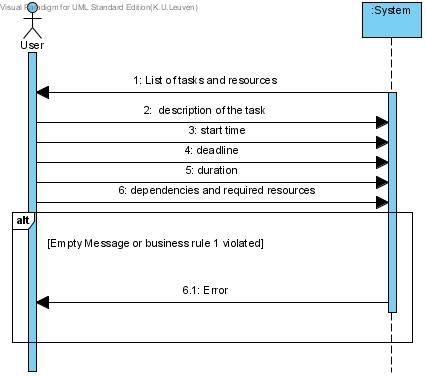
\includegraphics[scale=0.5]{images/ssd_create_task.jpg}
					\end{center}
					\caption{System Sequence Diagram describing the creation of a task}
				\end{figure}
			\subsubsection{Removing Tasks}
			When a task is to be removed. It first has to check how that will affect other entities in the system. Is a Task still required by other Tasks in a dependency?
			If this is the case. The user will receive an error message and is asked how he wants to proceed: Cancel the operation or delete all the dependent tasks.
			\begin{figure}[H]
				\begin{center}
					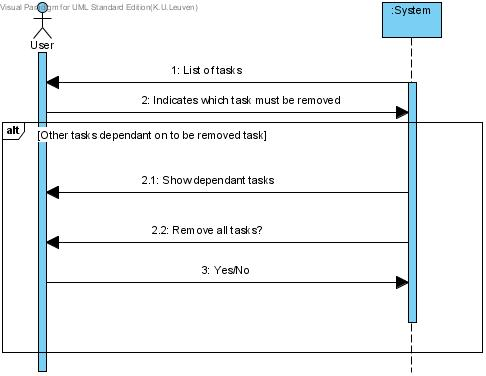
\includegraphics[scale=0.5]{images/ssd_remove_task.jpg}
				\end{center}
				\caption{System Sequence Diagram describing the removal of a task}
			\end{figure}
			\subsubsection{Modifying Tasks}
			When modifying tasks, the system has to make sure the user follows all the rules described above. This is because the user has the option to change all of the schedule variables, dependencies and required resources.

			This means that the Business Rule has to be tested, as well as the Empty Description rule. Checking is also done on the task dependencies. For instance, it should not be possible to create a task A, dependent on task B. And modify task B to be dependent on task A. This would create a dependency loop.\\
			\begin{figure}[H]
				\begin{center}
					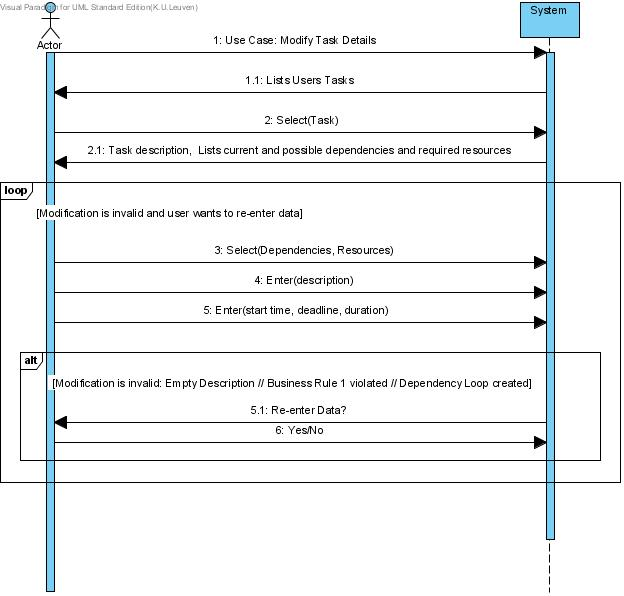
\includegraphics[scale=0.5]{images/ssd_modify_task.jpg}
				\end{center}
				\caption{System Sequence Diagram describing the editing of a task}
			\end{figure}
			 \subsubsection{Updating a Task status}
			Updating a status of a task is integrated in modifying a task, but requires special attention as many different rules apply when adjusting the status of a Task.

			Updating the status can directly reflect the status of dependent tasks. When a task was marked Successful, but is reverted to Failed or Unfinished the user will be asked to update the status of all dependent tasks or leave everything including this tasks status unchanged. This is because may have to revert back to Failed or Unfinished because they depended on the successful completion of this task.
			\emph{
			\subsection{Getting a task overview}		
			When asking for a overview of tasks, it is sometimes easy to sort and/or filter tasks in a different manner. That way you can get a better overview.\\
			We provided a handy interface for this in the way of a loop. The user can choose how he wants his tasks sorted: by deadline of by duration. In case the user selects to sort the tasks by deadline, he is asked how many tasks are to be shown. Is duration selected, a minimum and maximum duration is asked. It's made particulary easy to alter and/or add sorting and filtering methods.\\}
			\begin{figure}[H]
				\begin{center}
					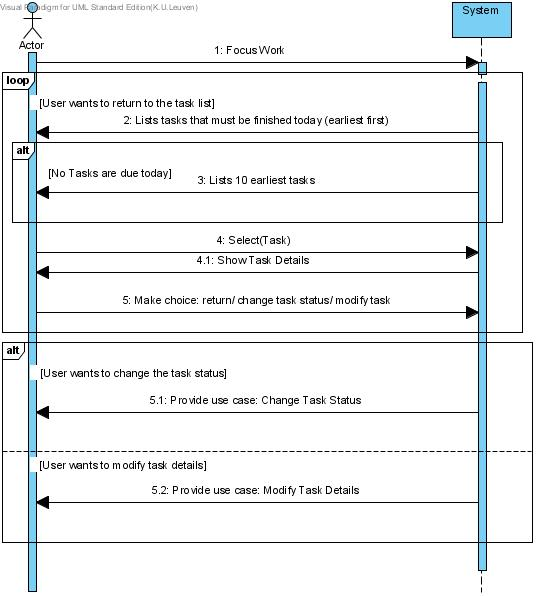
\includegraphics[scale=0.5]{images/ssd_focus_work.jpg}
				\end{center}
				\caption{System Sequence Diagram describing the overview of all tasks}
			\end{figure}
			
			
			\begin{figure}[H]
				\begin{center}
					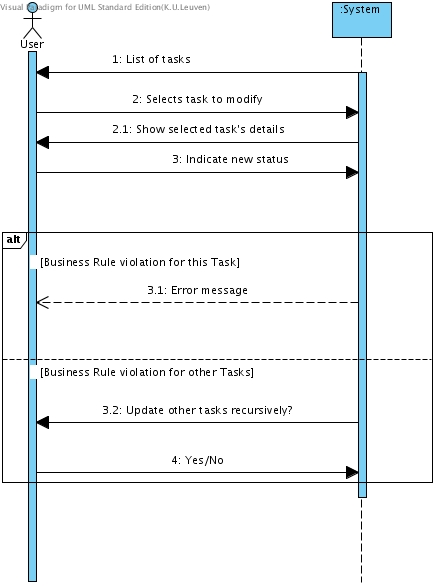
\includegraphics[scale=0.5]{images/ssd_update_task.jpg}
				\end{center}
				\caption{System Sequence Diagram describing the updating of the status of a Task}
			\end{figure}
		\subsection{Resource Management}
			\subsubsection{Creating Resources}
			A user can create a resource. When this resource is created, it is added to the system and stored there for later use.
			The system will only check for a valid description. This means the description can not be empty.

			Once created, the resource is available for binding to Tasks, or Reservations.
			\begin{figure}[H]
				\begin{center}
					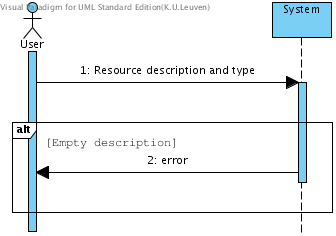
\includegraphics[scale=0.5]{images/SSD_Create_Resource.png}
				\end{center}
				\caption{System Sequence Diagram describing the creating of a new resource}
			\end{figure}
			\subsubsection{Remove Resource}
			A Resource can be removed. However, the system will first check it's dependency's with Task objects and/or Reservations.
			If the Resource is required by any of these, the system can not remove the Resource.
			\begin{figure}[H]
				\begin{center}
					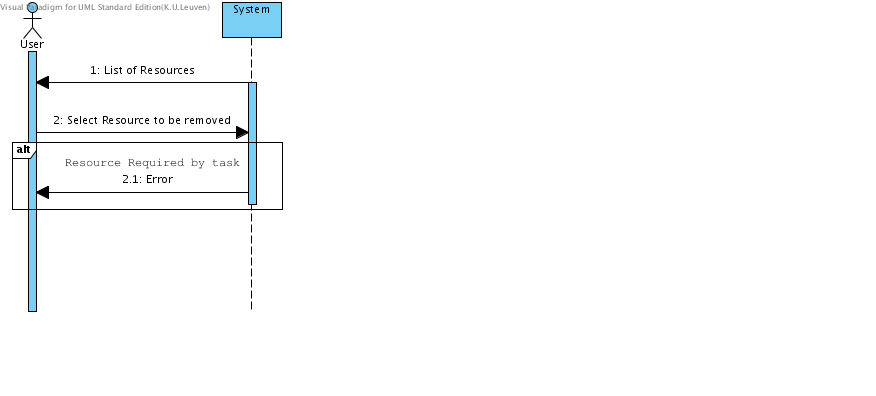
\includegraphics[scale=0.5]{images/SSD_Remove_Resource.png}
				\end{center}
				\caption{System Sequence Diagram describing the removing of a resource}
			\end{figure}
		\subsection{Reservations}
			\subsubsection{Create Reservations}
			Once a Resource is created, the User has the option to make a Reservation for that Resource.
			When creating a Reservation, the user is asked for the period of time he wants to make the Reservation after being shown a list of current Reservations for the Resource.

			After the user enters this data, the system controls the entered data to see if it does not conflict with previous Reservations.
			\begin{figure}[H]
				\begin{center}
					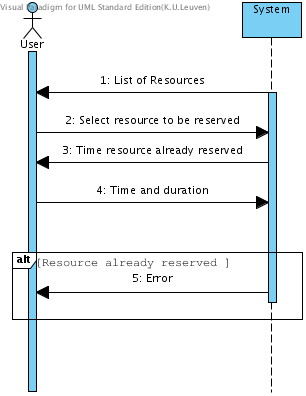
\includegraphics[scale=0.5]{images/SSD_Make_Resource_Reservation.png}
				\end{center}
				\caption{System Sequence Diagram describing the making of a reservation}
			\end{figure}
		\subsection{Project Management}
			\subsubsection{Create Project}
			A project can be created. A project can contain many Tasks, but does not have to. Our assumption is that at least one User is allocated to a Project, but several Users can subscribe.
			The system asks the user for a short description of that Project. If this description was not empty, the system creates the Project.
			\begin{figure}[H]
				\begin{center}
					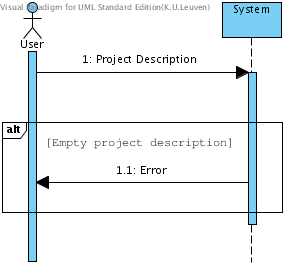
\includegraphics[scale=0.5]{images/SSD_Create_Project.png}
				\end{center}
				\caption{System Sequence Diagram describing the creating of a project}
			\end{figure}
			\subsubsection{Remove Project}
			A project can be removed without too many details. If the user wants to remove a project, all of the tasks connected to that project are removed. The user simply selects a Projects and all of the underlying tasks/dependent tasks are removed with it.
			\begin{figure}[H]
				\begin{center}
					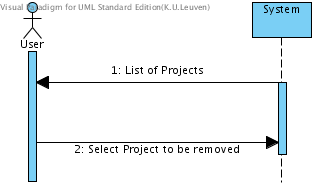
\includegraphics[scale=0.5]{images/SSD_Remove_Project.png}
				\end{center}
				\caption{System Sequence Diagram describing the removing of a project}
			\end{figure}
		\subsection{User Interface}
			\begin{figure}[H]
				\begin{center}
					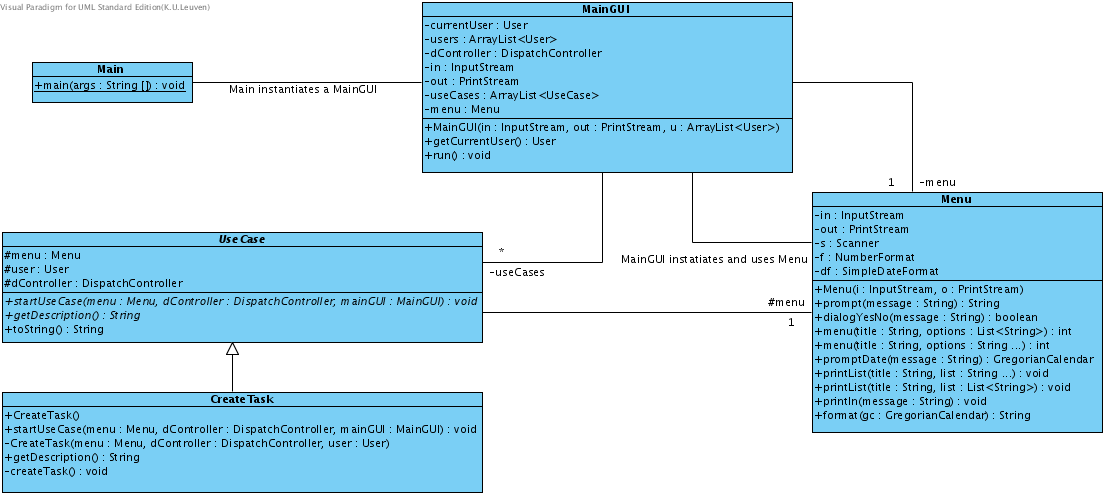
\includegraphics[width=1.0\textwidth]{images/gui.png}
				\end{center}
				\caption{Class diagram of the GUI}
			\end{figure}
			The project uses a text based UI. All use case are handled by a subclass of the abstract UseCase class, in the figure the use case for Create Task is given as example. MainGUI keeps a list of instance of these use cases. When the user initiates a use case MainGUI calls the corresponding use case, passing on the dispatch controller which will be discussed later, the use case then creates a new instance of itself with all field initialized to handle the rest of the use case. The class Menu handles the actual communication with the user through the console, formatting all the in and output.
			
	\section{Package Communication}
	       The whole project is divided in four big packages. These packages are 'model', 'controller' and 'gui'. The last package is 'test', which has been separated from the rest of the project for obvious reasons.
       
        We chose to create these packages so everything would be separated from each other. It would be bad practice to let the GUI access the model in a direct way, since this would mean even a small change could result in massive changes throughout the GUI. 
        
        This is where the controllers come in. They offer a way of communicating with the model. They basically contain a set of functionalities that are used throughout the program. These will then make the correct calls to the model. This way everything is handled without using direct calls, creating a more persistent system against changes throughout the model.
        
        All these controllers are finally instantiated inside one big container called the dispatch controller. This controller enables the GUI to just instantiate one controller. Its constructor will take care of the rest. The other controllers are stored inside it and can be accessed by calling the correct getters. All the controllers can then easily be passed along the different views using this one object.

	\section{Class Descriptions}
		
			\subsection{User}
			At first, we intended the User class to be responsible for the creation of Projects and Tasks, because a User object contains a list of Tasks and Projects that belong to that User. In the end, we chose not to do so. We felt that that the indirection was not necessary and that it might not benefit the cohesion of the User class.

			While not described in the project assignment, we assumed the system could become a multi-user system in the next iteration(s). We therefore based our design on this.

			Every User object is responsible for keeping track of the Projects and Tasks that belong to him. The system can ask the User object to return a list of these Projects or Tasks.

			\subsection{Task manipulation}
			%Design uitleggen. Ook de GRASP patterns erbij zetten
			Tasks are collected in the User. They contain a list of Resources the User might require to execute the Task.
			A Task has attributes which define it's own description, a Start and End time as well as a Duration.
			Also, a Task has a list of Tasks on which the Task may depend. This means the status of the Task at hand is dependent on the Status of it's dependent Tasks.\\
			Keeping Low Coupling and High Cohesion in mind, Task has the following responsibilities:
			\begin{itemize}
				\item{Keeping track of its name, start date, due date, duration and status}
				\item{Keeping track of the resources required to execute the task}
				\item{Keeping track of its dependencies. A dependency is implemented as a double binding, so the Tasks on both ends should be kept consistent}
				\item{Checking for the business rule 1 and preventing the construction of loops in the dependency scheme}
				\item{Updating the status of dependent tasks when necessary}
			\end{itemize}
			A Task is not an Information Expert or Creator of Resources. As described in the next chapter, a Resource has its own management.
			We do feel it is necessary for the Task to know about its Resources.\\
			However, a Task is Information Expert about Task itself. Therefore, we felt that the Task class should be responsible for enforcing business rule 1, preventing the construction of dependency loops, and updating the status of dependent tasks when necessary (as described in the use case 'update task status').
			
			While designing, it was suggested that perhaps the Task class has two distinct responsibilities this way: one concerning its own details, and one concerning the way it interacts with other Tasks in the dependency graph. In the end, we chose to stick to one single Task class, as we felt that the cohesion of this class was sufficiently high.
			
		
			\subsubsection{Task dependency manager}
				\emph{
			In the second iteration, we chose to have a second object manage the dependencies of tasks. A new class TaskDependencyManager was created. A Task object aggregates an instance of TaskDependencyManager at all times. All operations that concern only dependencies are delegated to this object.}
			
			\emph{
			On one hand, this creates a strong coupling between the Task and the TaskDependencyManager classes. On the other hand, we felt that the Task class was getting too bloated, and that it was responsible for too many things. Delegating some operations to the TaskDependencyManager helps to improve the cohesion of the Task class.}
			
			\begin{figure}[h]
			\begin{center}
			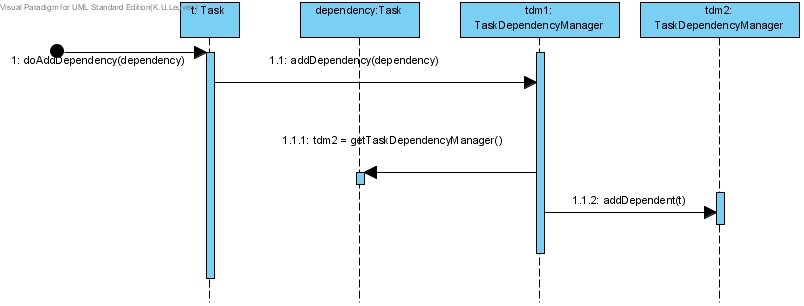
\includegraphics[scale=0.5]{images/doAddDependency}
			\end{center}
			\caption{\emph{Sequence diagram to add a dependency to a Task}}
			\end{figure}
			
			\emph{
			In the diagram is shown how adding a dependency to a Task works now. The Task object delegates this action
			to its TaskDependencyManager. The TaskDependencyManager then cooperates with the TaskDependencyManager of the second Task, to make sure the double binding is kept consistent.			
			Note: the diagram uses the operation 'doAddDependency()', not 'addDependency()'. This is because the operation 'addDependency()' is first delegated to the TaskState class. This is explained later in the report.}
			
			\subsection{Resource manipulation}
			%Design uitleggen. Ook de GRASP patterns erbij zetten
			Resources can be accessed via Tasks. This is because a Task can define which resources are required for that Task.
			However when a Resource is just created, or when a Task to which a Resource was allocated gets removed, the Resource will not be referenced to by any Task. The object would not exists.
			Therefore we decided that it was necessary to keep a reference of each Resource in a class with a static instance.

			A Resource itself is an Information Expert as well as a Creator for Reservations. We decided to put the responsibility of creating and storing Reservations in Resource because a Resource needs this information to check it's own availability, as displayed in the diagram 'Create Reservation'.
			\begin{figure}[H]
				\begin{center}
					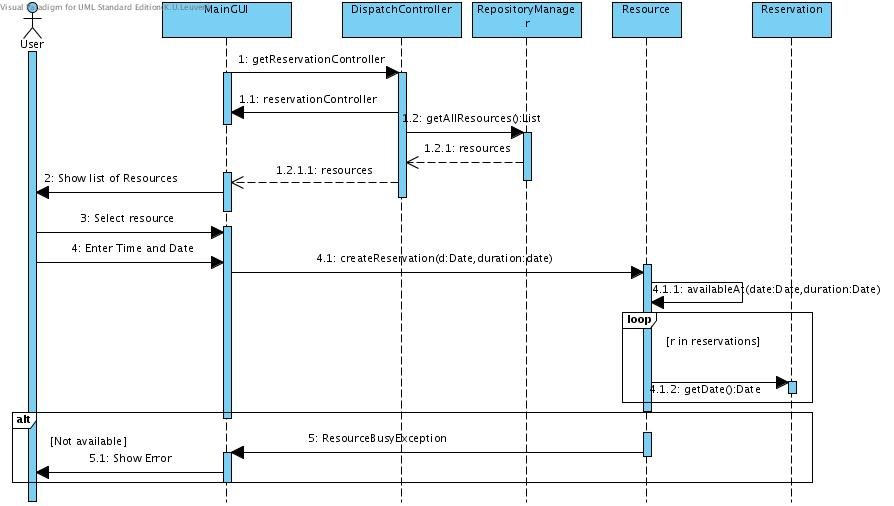
\includegraphics[scale=0.5]{images/create_reservation.jpg}
				\end{center}
				\caption{Create Reservation Sequence Diagram}
			\end{figure}

			As shown in the diagram , all the Resources are retrieved from the Singleton ResourceManager. The resource is responsible for keeping track of its reservations and checking whether it is available. When available the Resource itself creates the Reservation.
			
			The ResourceManager keeps track of all the resources, and is responsible for the construction or destruction of Resource objects. When the ResourceManager tries to destroy a Resource, it is the Resource's responsibility to check if this operation is allowed. According to use case 'Remove Resource' this operation will fail if any task requires the resource. The Resource object will then hand an exception to the ResourceManager, which is responsible for communicating it to the GUI. A sequence diagram of this operation is shown in figure 'Remove Sequence Diagram'.
			
			\begin{figure}[H]
			\begin{center}
			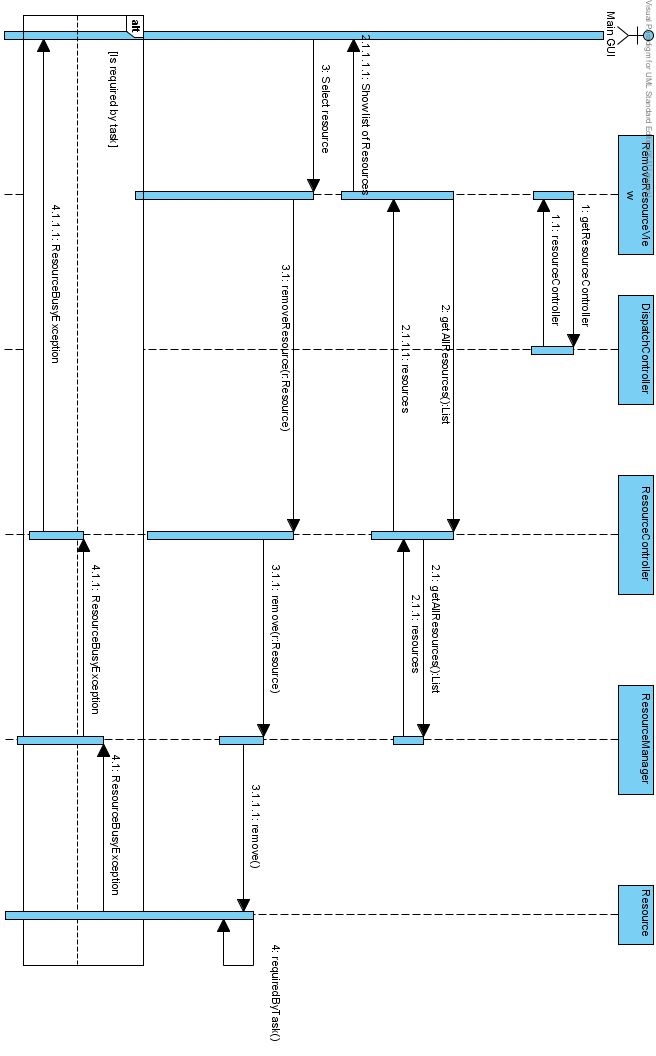
\includegraphics[scale = 0.5]{images/RemoveResource.png}
			\end{center}
			\caption{Remove Resource Sequence Diagram}
			\end{figure}
			

			The OO-structure is shown in the class diagram: Resource Class Diagram which contains all the necessary classes for the Resource subsystem.
			
			\begin{figure}[H]
				\begin{center}
					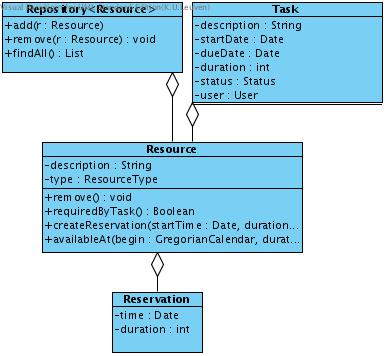
\includegraphics[scale=0.5]{images/resource_class_diagram.jpg}
				\end{center}
				\caption{Resource Class Diagram}
			\end{figure}
			
			
			\subsection{Project manipulation}
			When we assumed the project could become a multi-user application. We thought of Projects as a link between multiple Users and Tasks. Therefore, a Project can contain multiple Tasks, and multiple Users can be assigned to it.
			\begin{figure}[H]
				\begin{center}
					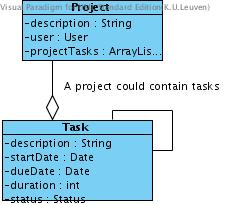
\includegraphics[scale=0.5]{images/project_class_diagram.jpg}
				\end{center}
				\caption{Project Class Diagram}
			\end{figure}
			
			The responsibilities of the Project class are as follows:
			\begin{itemize}
			\item Keeping track of its own details (description)
			\item Keeping track of the Tasks that are in the project
			\item Binding or removing Tasks from or to the project
			\end{itemize}

			When the application user creates a Project, he becomes a owner of that Project, this is how the User acts as a container of the Project Object. Tasks can be added to the Project however the User wishes to do this. However, it's not the User object that calls the Project constructor. It is our opinion that it is not the User's responsibility to create this object, rather then it's the Project's responsibility to aggregate the User.
			\begin{figure}[H]
				\begin{center}
					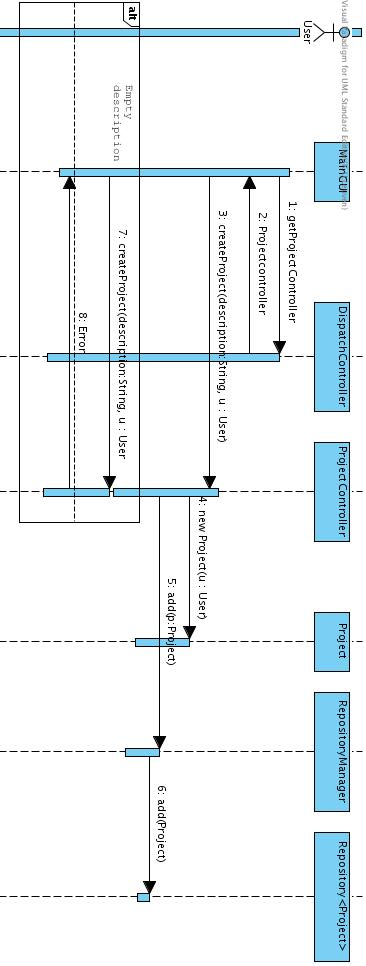
\includegraphics[scale=0.5]{images/create_project.jpg}
				\end{center}
				\caption{Create Project Sequence Diagram}
			\end{figure}
			Therefore, it's the Project's constructor that gets an argument User. This User object is then asked to add Project to it's list of Projects.
			\begin{figure}[H]
				\begin{center}
					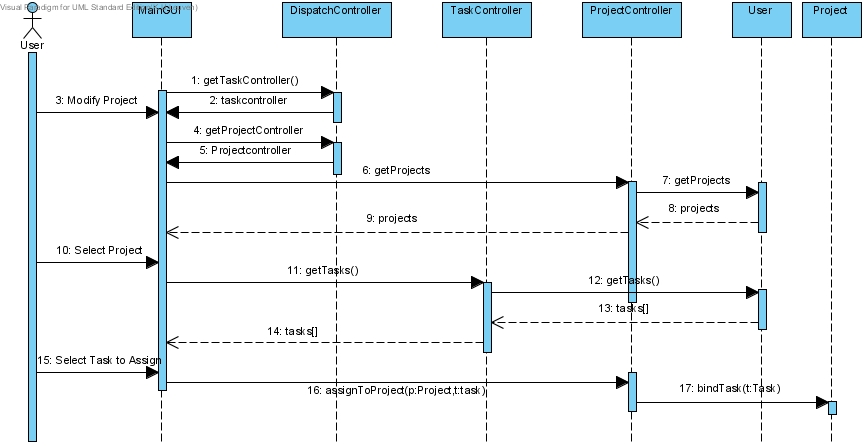
\includegraphics[scale=0.5]{images/assign_task_to_project.jpg}
				\end{center}
				\caption{Assign Task to Project Sequence Diagram}
			\end{figure}
			It is also the Project's responsibility to bind a Task to the Project. We feel that this direction should be maintained because a Project 'contains' or 'aggregates' a Task. This binding is done in the Project's constructor.	
	
	\section{Software Structures}
		\subsection{Task states}
		Hier komt iets over het gebruik van State pattern. Ook observer zou ik hier zetten
		\subsection{Task overview}
		Focus dinges
		\subsection{Linking Tasks by dependency}
		Uitleggen hoe tasks gelinked worden zonder te veel binding = taskdependencymanager
		\subsection{Time representation}
		Clock uitleggen, nut en werking
		\subsection{Collecting data}
		Repositories, waarom en hoe
		
	\section{Software Initialization}
	When the program is started, the first thing that is taken care of is the instantiation of the dispatch controller.
	
	After that, an XML parser object is created to retrieve all the supplied information. The dispatch controller, together with the location of the XML file, are passed to the constructor of the parser. After this it can finally start parsing.
	
	The first thing it will do is find all the resources in the file. It will then instantiate the ResourceManager singleton and start adding these resources. Once that has been completed, it will start looking for projects. It will create all the found instances. After this it looks for all the tasks and, once again, creates them all. Finally all the tasks, resources and projects are bound according to the specifications in the XML file. It will finally return the user object found in the file.
	
	After this the GUI is instantiated. The user object from before is passed along with its constructor and then starts listening for any input. 
	
	The system has now fully started and is ready for use.	
	
	
	\section{Testing}
		\subsection{Technology}
		We decided to use JUnit4 for testing.
		JUnit4 has a few advantages compared to JUnit3. It uses annotations to define a Test. This gives the developer an easy solution to testing for Exceptions.
		\subsection{Testing Approach}
		We decided to go for a defensive and multi-level testing approach.
		By multi-level we mean that we test both methods in Model classes (such as User, Task, Resource etc.) as well as testing the Controllers that call these methods (TaskController, ResourceController etc). 
		This way we get a good view on where errors are: model, controller or view.\\
		We also tested most methods for both cases. This means that we test both failure and succession of a method. Testing only for success does not guarantee a correct Exception is thrown, or success in all cases.
	\section{Project Management}
		\subsection{Planning}
		The planning of our Team Assignment had the following planning:\\
		\begin{tabular}{p{200 pt}|c|c}
		Activity & From & To\\
		\hline
		First meeting \& Discussion of our views on the project & 9/10/2009 & 9/10/2009\\ \hline
		Creation of a draft class diagram \& working out System Sequence Diagrams & 9/10/2009 & 12/10/2009\\ \hline
		First meeting with our advisor. & 12/10/2009 & 12/10/2009\\ \hline
		Individual rework of Class Diagram & 12/10/2009 & 14/10/2009\\ \hline
		Comparing results and creation of definitive Class Diagram & 14/10/2009 & 14/10/2009\\ \hline
		Creation of Sequence Diagrams & 14/10/2009 & 16/10/2009\\ \hline
		Development of Model classes and Controller classes. Building of GUI structure & 16/10/2009 & 19/10/2009\\ \hline
		Code review by team and rewriting certain functionality's & 19/10/2009 & 26/10/2009\\ \hline
		Start writing report \& finishing UML diagrams & 24/10/2009 & 27/10/2009\\ \hline
		\end{tabular}
		\subsection{Teamwork}
		We focused on a close teamwork. We started the project with a team discussion on how everyone saw the project and interpreted the assignment. This gave the team a general perspective and good grasp on how we wanted to implement it.\\
		We have 3 weekly physical meetings, where 1 would be with our team advisor. In these meetings, we discussed what everyone had done in the past days. Whenever somebody was unclear, or the group had doubts about which method or pattern would be the best to use, time was never an issue to come to a general solution that seemed best to everyone.\\
		We also used several team collaboration tools provided by Google such as Google Code and Google Groups. This gave advantages such as a mailing list, subversion with the option to review code at each revision, issue lists and hosted files.\\
		We tried to keep all the information as centralized as possible by using a separate Subversion repository for the Visual Paradigm file. This way every team member always had the most up to date diagrams available.\\
		Development of the project was divided in 4 groups of functionality: Controllers, Models, View and Testing. Each member of the team was assigned one of these tasks. Steven Thuriot took on Controllers and the parsing of XML, Kwinten Missiaen Models, Koen Van den dries the View and Bart Vangeneugden Testing. The report was structured and drafted by Bart Vangeneugden however every team member wrote about the part of development he was responsible for.\\
		We had a total of 18 hours meeting physically for the project. Besides that every group member worked at home. A short estimate follows:\\
		 \begin{tabular}{l|l}
		Member & Time(+/-)\\ \hline
		Kwinten Missiaen & 30\\
		Steven Thuriot & 25\\
		Koen Van den dries & 23\\
		Bart Vangeneugden & 25\\
		\end{tabular}
	\section{Self-Evaluation}
	It is our opinion that we had a great team effort. However, we can improve. In this iteration we were too eager to get a first version of Class- and other diagrams ready. It would have been a better choice to make a good class-per-class analysis before drawing.\\
	To conclude we had no real problems regarding teamwork. Also we learned a lot about project organization.
\end{document}
